\documentclass[../main]{subfiles}

\begin{document}

\part*{第1回}

\section{静電場}

\subsection{電荷}

{\bf 電荷}は,観測者の座標系によらず保存する.
物体のもつ電荷の大きさはある量の整数倍であることが知られており,それを{\bf 電気素量}といい,記号eで表す.
電気素量の値は$1.602 \times 10^{-19}{\rm C}$であることが1909年にR.Millikanらによって計測された.
電気素量は電子の電荷の絶対値と陽子の電荷に等しい.
以降我々が静電場を議論する上では,{\bf 点電荷},すなわち{\bf 数学的な一点に有限の電荷が集中しているモデル},が有効である.

\subsection{Coulombの法則}


互いに静止している2つの点電荷の間に働く力({\bf Coulomb力})を考える.\\
力の大きさ$F$は以下の式で表される.\\
\begin{equation}
F=\frac{|q_{1}q_{2}|}{4\pi \varepsilon_{0} r^2}
\end{equation}
Coulomb力は{\bf 作用・反作用の法則}を満たすので,互いの点電荷に働く力の大きさは等しく,向きは反対方向である.\\
力の向きは$q_{1}$と$q_{2}$を通る直線上になる.
この力が引力か斥力か,は$q_1q_2$の符号によって決まる.すなわち,

\begin{figure}[htbp]
 \begin{center}
  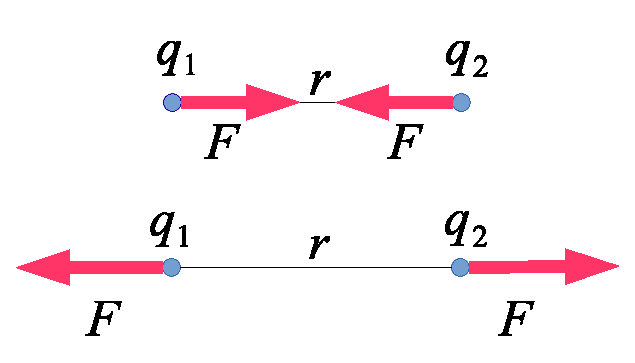
\includegraphics[width=80mm]{1.1.eps}
 \end{center}
 \caption{}
 \label{fig:one}
\end{figure}


\begin{equation}
\left \{
\begin{array}{l}
qe1q_2 <0のとき引力\\
q_1q_2 >0のとき斥力\\
\end{array}
\right.
\end{equation}
となる.\\
さて,ここで万有引力とCoulomb力の比はどのくらいになるのか計算する.\\
例として,二つの陽子が距離$r$だけ離れて静止している状況を考える.

\begin{equation}
\frac{\mbox{Coulomb力}}{\mbox{万有引力}} =  \frac{\frac{q^2}{4\pi \varepsilon_0}}{G\frac{m^2}{r^2}} 
= \frac{1}{4 \pi \varepsilon_0}\frac{q^2}{Gm^2}
\end{equation}


\begin{equation}
\left \{
\begin{array}{l}
\frac{1}{4 \pi \varepsilon_0}=9.0 \times 10^9 [{\rm Nm^2C^{-2}}] \\
陽子の電荷(電気素量) \, 1.6 \times 10^{-19} [{\rm C}] \\
陽子の質量 \, 1.7 \times 10^{-27} [{\rm kg}] \\
万有引力定数 \, 6.7 \times 10^{-11} [{\rm m^3s^{-2}kg^{-1}}]
\end{array}
\right.
\end{equation}
(4)の値を用いて計算をすると,結果は\\
\begin{equation}
\frac{\mbox{Coulomb力}}{\mbox{万有引力}} \simeq 10^{36} 
\end{equation}
となり,Coulomb力の大きさ(あるいは万有引力の小ささ)が分かる.\footnote{これは陽子の例ですが,他の粒子について計算してみてもCoulomb力の大きさが分かるでしょう.}\\


ここまで直線上に静止した点電荷について考えてきたが,今度は空間に自由に配置された点電荷について考えるために,Coulomb力のベクトルによる表記を学ぶ.\\

\begin{figure}[htbp]
 \begin{center}
  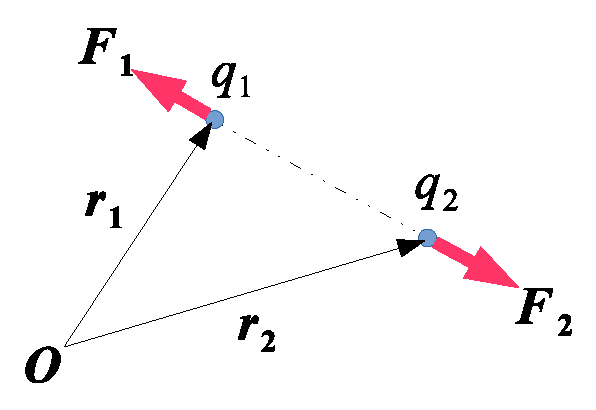
\includegraphics[width=80mm]{1.2.eps}
 \end{center}
 \caption{}
 \label{fig:one}
\end{figure}

点電荷$q_2$から$q_1$に働く力${\bf F_1}$をつくる,
Coulomb力の大きさは式(1)で表されるので,これに向きの情報を付加するために,直線方向の単位ベクトルを作ればよい.
点電荷$q_2$から$q_1$に向かうベクトルは${\bf r}_1-{\bf r}_2$である.
点電荷間の距離は, $|{\bf r}_1-{\bf r}_2|$である.\\
したがって単位ベクトルは
$\frac{{\bf r}_1-{\bf r}_2}{|{\bf r}_1-{\bf r}_2|}$とわかる.
式(1)で$r$を$|{\bf r}_1-{\bf r}_2|$に書き直せば,

\begin{eqnarray}
{\bf F}_1 =  \frac{q_{1}q_{2}}{4\pi \varepsilon_{0} |{\bf r}_1-{\bf r}_2|^2}\frac{{\bf r}_1-{\bf r}_2}{|{\bf r}_1-{\bf r}_2|} = \frac{q_{1}q_{2}}{4\pi \varepsilon_{0}}\frac{{\bf r}_1-{\bf r}_2}{|{\bf r}_1-{\bf r}_2|^3}
\end{eqnarray}
いま,$|q_1q_2|$の絶対値を外したが,それによって力の方向は(2)を満たすようになる.
(6)が,点電荷$q_2$から$q_1$に働くCoulomb力のベクトル表記である.
逆に,点電荷$q_1$から$q_2$に働く力${\bf F_2}$は,式(6)で$r_1$と$r_2$を入れかえて,

\begin{eqnarray}
{\bf F}_2 = \frac{q_{1}q_{2}}{4\pi \varepsilon_{0}}\frac{{\bf r}_2-{\bf r}_1}{|{\bf r}_2-{\bf r}_1|^3}
\end{eqnarray}
さて,式(6)と式(7)の和をとると,

\begin{eqnarray}
{\bf F}_{1}+{\bf F}_{2}={\bf 0}
\end{eqnarray}
これはCoulomb力に{\bf 作用・反作用の法則}が成り立つことを示している.

Coulomb力には{\bf 重ね合わせの原理}が成り立つ.
静電場における{\bf 重ね合わせの原理}とはすなわち,\\
{\bf 複数の点電荷が配置されている空間において,ある点電荷が他の点電荷集団から受ける力は,その点電荷と個々の点電荷との間に働く力(二体力)の和に等しい}.\\

\begin{figure}[htbp]
 \begin{center}
  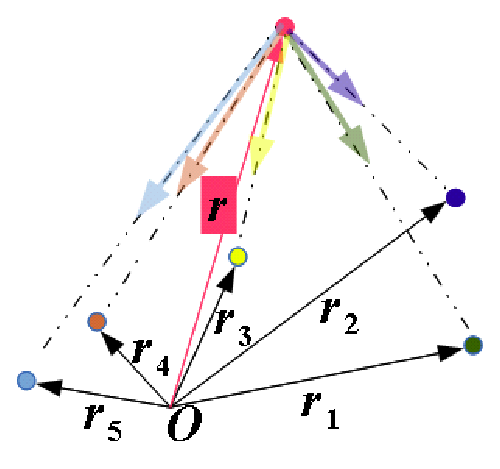
\includegraphics[width=60mm]{1.3.eps}
 \end{center}
 \caption{}
 \label{fig:one}
\end{figure}
位置${\bf r}_{i}$ ($i$ = 1,2,3...)に電荷$q_i$の点電荷が配置,固定されている空間を考える.\\
位置{\bf r}に電荷$q$の点電荷を配置するとき,点電荷$q_i$から受ける力${\bf F}_i$は,式(6),(7)と同様に考え,
\begin{eqnarray}
{\bf F}_{i} = \frac{qq_{i}}{4\pi \varepsilon_{0}}\frac{{\bf r}-{\bf r}_i}{|{\bf r}-{\bf r}_i|^3}
\end{eqnarray}
点電荷$q$が電荷集団から受ける力は,重ね合わせの原理から,

\begin{eqnarray}
{\bf F}=\sum^{}_{i}{\bf F_{i}}=\sum^{}_{i}\frac{qq_{i}}{4\pi \varepsilon_{0}}\frac{{\bf r}-{\bf r}_i}{|{\bf r}-{\bf r}_i|^3}
=q\sum^{}_{i}\frac{q_{i}}{4\pi \varepsilon_{0}}\frac{{\bf r}-{\bf r}_i}{|{\bf r}-{\bf r}_i|^3}
\end{eqnarray}

\subsection{電場}

式(10)で,電荷集団は固定されていて動かない(静的)であるから,新たに
\begin{eqnarray}
\sum^{}_{i}\frac{q_{i}}{4\pi \varepsilon_{0}}\frac{{\bf r}-{\bf r}_i}{|{\bf r}-{\bf r}_i|^3} = {\bf E}({\bf r})
\end{eqnarray}
として, 電気素量の電荷をもつ点電荷を,空間の位置{\bf r}に配置したとき,その電荷にはたらくCoulomb力を表す${\bf E}({\bf r})$を導入する.これを,位置{\bf r}における{\bf 電場}と呼ぶ.
これによって式(10)は
\begin{eqnarray}
{\bf F}({\bf r})= q{\bf E}({\bf r})
\end{eqnarray}
電荷は位置{\bf r}によらないから,式(12)を見ると
Coulomb力{\bf F}({\bf r})に重ね合わせの原理が成り立つということは,電場${\bf E}({\bf r})$にも重ね合わせの原理が成り立つことがわかる.

最後に,電場の性質について述べる.
電場は電荷を空間の任意の位置に配置した時,それが空間の各位置でどのような力を受けるかを表す.力はベクトルであるから,式(12)から位置{\bf r}における電場もベクトルである.電荷は任意の位置に配置できるから,空間のあらゆる位置に電場のベクトルが存在することになり,空間がベクトルで埋め尽くされているということになる.このような性質から,電場は{\bf ベクトル場}\footnote{対応する言葉に{\bf スカラー場}があり,これは空間の各点にスカラー値を対応させた場である.温度分布や液体の濃度分布などが好例.}である.
1.2節まではCoulomb力を,離れた電荷間を時間を介さずに伝わる力であると考えても良かった.このような考え方を{\bf 遠隔作用}という.しかし電場を導入したいま,Coulomb力はあらかじめ空間に存在する電場を介して伝わるという考え方ができるようになった.このような考え方を{\bf 近接作用}という.
結論としては,Coulomb力は近接作用の力である.\footnote{このことは講義が進むにつれて明らかになるでしょう.}
電場の視覚表現は{\bf 電気力線}によってなされる.電気力線は,{\bf 向きづけられた曲線群で,各点における接線が電場の向きと一致する},という性質をもつ.
図4は正電荷をもつひとつの点電荷から生じる電気力線である.
この電場と,絶対値が等しい負電荷をもつひとつの点電荷によって生じる電場が重ね合わさってできる電場の式(電気力線の形はよく知られているが)がどうなるかは,演習問題1を参考にされたい.

\begin{figure}[htbp]
 \begin{center}
  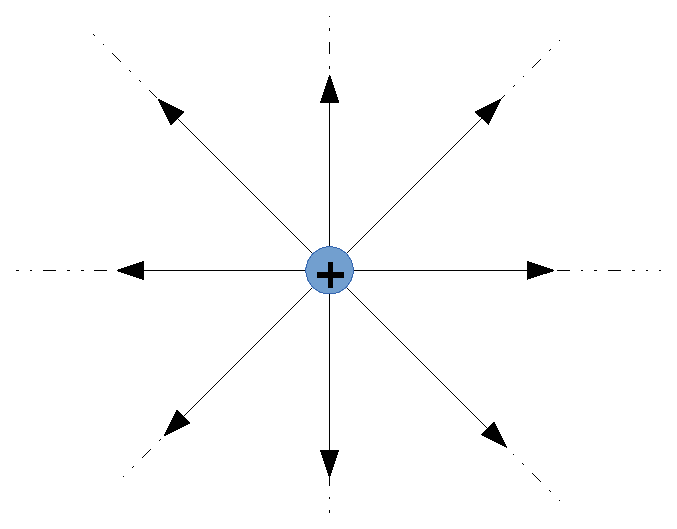
\includegraphics[width=60mm]{1.4.eps}
 \end{center}
 \caption{}
 \label{fig:one}
\end{figure}

\end{document}
